En esta sección, se presentan los resultados obtenidos al reproducir cada uno de
los experimentos de la sección anterior, es decir, los experimentos que los autores
presentan en su trabajo \cite{jsantos-amonteagudo-1-2014}.

Antes de todo, hay que tener en cuenta la componente aleatoria de la simulación. Esto es, por
la realización de sorteos de cara a ejecutar la mitosis u otra acción. En consecuencia, la aparición
de un marcador u otro, como se verá a continuación, provoca alteraciones en la simulación, de modo que
el comportamiento puede variar. En este caso, lo que se pretende es llegar a la misma conclusión que los autores,
por tanto, el análisis de los resultados propios debe hacerse con ese objetivo en mente.

\section{Influencia del parámetro \textit{Tasa de mutación base (m)}}

Las células de la simulación, y como se ha descrito en secciones previas, tienen asociado una propiedad que está relacionada con la aparición
de nuevas mutaciones durante la mitosis, este es, el parámetro \textit{tasa de mutación base} o $m$. En este experimento,
se pretende someter a la simulación a diferentes configuraciones de este parametros para estudiar qué
progresión presentan los tumores.

Se parte de una probabilidad de aparición de mutaciones baja, ya que, el sorte se efectua con una probabilidad de
$1/m$, por lo que, a mayor valor del parámetro $m$, menor probabilidad de que ocurre. En este caso, se
realizan tres simulaciones, para $m=10000$, $m=1000$ y $m=100$.

\subsection{Experimento 1: Tasa de mutación base igual a 10.000}

En esta simulación, se obtienen tres gráficas respecto de la misma. En la primera, se observa la progresión
en el número de células sanas frente a células cancerosas.

En cuanto al número de células de uno u otro tipo, se observa una progresión bastante similar a la obtenida por los autores.
Por un lado, el número de células sanas crece muy rápido y ocupa el $90\%$ del espacio en torno a las $300$ iteraciones. Por otro lado,
el número de células cancerosas presenta una progresión similar con un repunte leve en torno a la iteración $300$ con un crecimiento muy leve.


\begin{figure}[h]
\centering
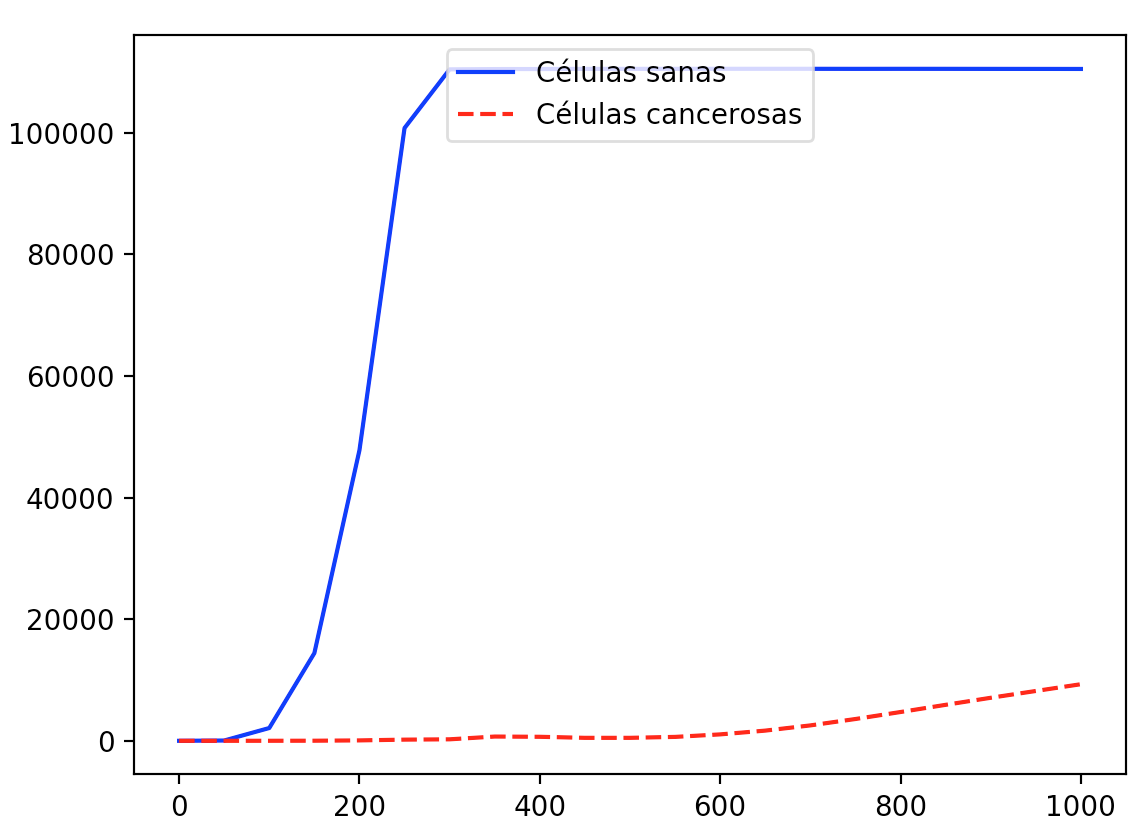
\includegraphics[scale=0.6]{figures/experiments/exp1/healthvscarcino}
\caption{Completar.}
\end{figure}

En cuanto a los marcadores presentes y a su progresión, se observan algunas diferencias. Completar.

\begin{figure}[h]
\centering
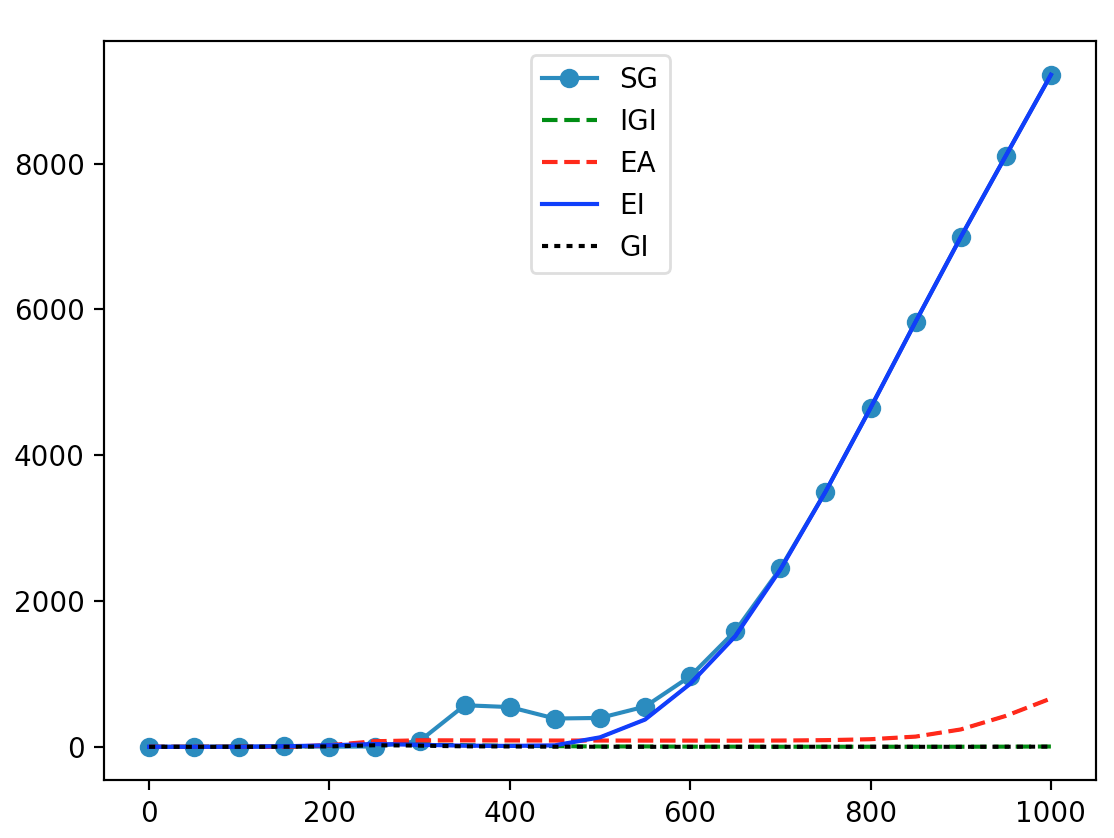
\includegraphics[scale=0.6]{figures/experiments/exp1/mutations}
\caption{Completar.}
\end{figure}

Lorem ipsum dolor sit amet, consectetur adipisicing elit, sed do eiusmod tempor incididunt ut labore et dolore magna aliqua.
Ut enim ad minim veniam, quis nostrud exercitation ullamco laboris nisi ut aliquip ex ea commodo consequat.
Duis aute irure dolor in reprehenderit in voluptate velit esse cillum dolore eu fugiat nulla pariatur.
Excepteur sint occaecat cupidatat non proident, sunt in culpa qui officia deserunt mollit anim id est laborum.

\begin{figure}[h]
\centering
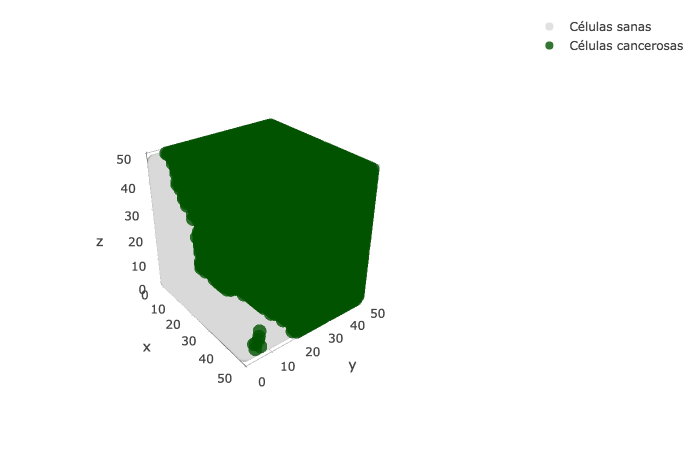
\includegraphics[scale=0.6]{figures/experiments/exp1/grid}
\caption{Completar.}
\end{figure}

Lorem ipsum dolor sit amet, consectetur adipisicing elit, sed do eiusmod tempor incididunt ut labore et dolore magna aliqua.
Ut enim ad minim veniam, quis nostrud exercitation ullamco laboris nisi ut aliquip ex ea commodo consequat.
Duis aute irure dolor in reprehenderit in voluptate velit esse cillum dolore eu fugiat nulla pariatur.
Excepteur sint occaecat cupidatat non proident, sunt in culpa qui officia deserunt mollit anim id est laborum.

\subsection{Experimento 2: Tasa de mutación base igual a 1.000}

Lorem ipsum dolor sit amet, consectetur adipisicing elit, sed do eiusmod tempor incididunt ut labore et dolore magna aliqua.
Ut enim ad minim veniam, quis nostrud exercitation ullamco laboris nisi ut aliquip ex ea commodo consequat.
Duis aute irure dolor in reprehenderit in voluptate velit esse cillum dolore eu fugiat nulla pariatur.
Excepteur sint occaecat cupidatat non proident, sunt in culpa qui officia deserunt mollit anim id est laborum.

\begin{figure}[h]
\centering
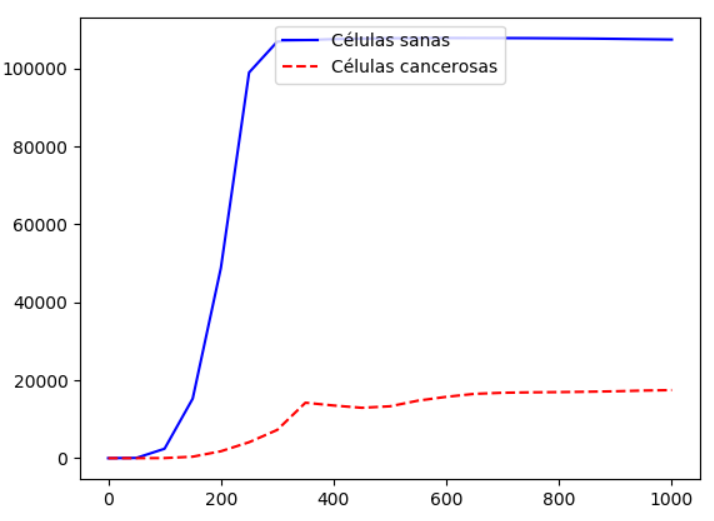
\includegraphics[scale=0.8]{figures/experiments/exp2/healthvscarcino}
\caption{Completar.}
\end{figure}

Lorem ipsum dolor sit amet, consectetur adipisicing elit, sed do eiusmod tempor incididunt ut labore et dolore magna aliqua.
Ut enim ad minim veniam, quis nostrud exercitation ullamco laboris nisi ut aliquip ex ea commodo consequat.
Duis aute irure dolor in reprehenderit in voluptate velit esse cillum dolore eu fugiat nulla pariatur.
Excepteur sint occaecat cupidatat non proident, sunt in culpa qui officia deserunt mollit anim id est laborum.

\begin{figure}[h]
\centering
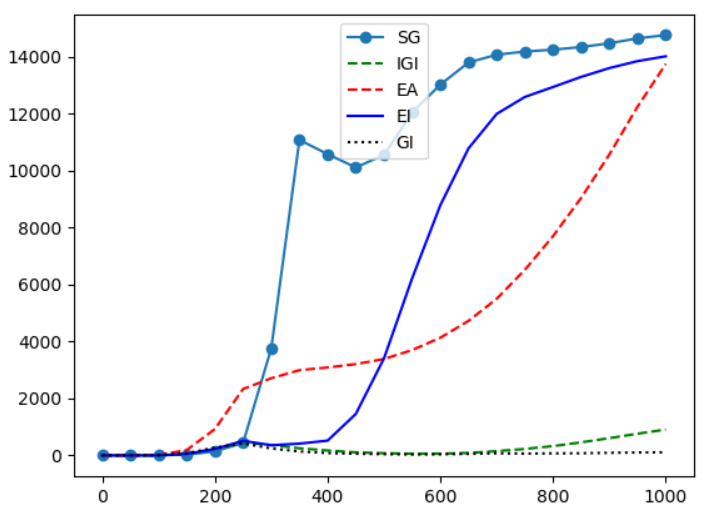
\includegraphics[scale=0.8]{figures/experiments/exp2/mutations}
\caption{Completar.}
\end{figure}

Lorem ipsum dolor sit amet, consectetur adipisicing elit, sed do eiusmod tempor incididunt ut labore et dolore magna aliqua.
Ut enim ad minim veniam, quis nostrud exercitation ullamco laboris nisi ut aliquip ex ea commodo consequat.
Duis aute irure dolor in reprehenderit in voluptate velit esse cillum dolore eu fugiat nulla pariatur.
Excepteur sint occaecat cupidatat non proident, sunt in culpa qui officia deserunt mollit anim id est laborum.

\begin{figure}[h]
\centering
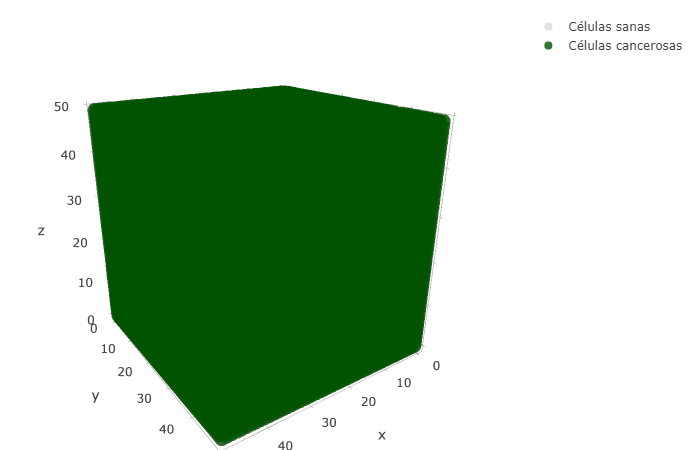
\includegraphics[scale=0.6]{figures/experiments/exp2/grid}
\caption{Completar.}
\end{figure}

Lorem ipsum dolor sit amet, consectetur adipisicing elit, sed do eiusmod tempor incididunt ut labore et dolore magna aliqua.
Ut enim ad minim veniam, quis nostrud exercitation ullamco laboris nisi ut aliquip ex ea commodo consequat.
Duis aute irure dolor in reprehenderit in voluptate velit esse cillum dolore eu fugiat nulla pariatur.
Excepteur sint occaecat cupidatat non proident, sunt in culpa qui officia deserunt mollit anim id est laborum.

\subsection{Experimento 3: Tasa de mutación base igual a 100}

Lorem ipsum dolor sit amet, consectetur adipisicing elit, sed do eiusmod tempor incididunt ut labore et dolore magna aliqua.
Ut enim ad minim veniam, quis nostrud exercitation ullamco laboris nisi ut aliquip ex ea commodo consequat.
Duis aute irure dolor in reprehenderit in voluptate velit esse cillum dolore eu fugiat nulla pariatur.
Excepteur sint occaecat cupidatat non proident, sunt in culpa qui officia deserunt mollit anim id est laborum.

\begin{figure}[h]
\centering
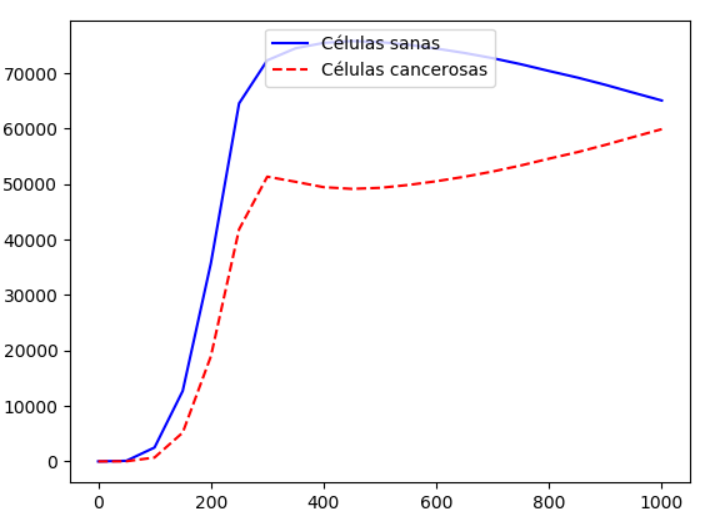
\includegraphics[scale=0.8]{figures/experiments/exp3/healthvscarcino}
\caption{Completar.}
\end{figure}

Lorem ipsum dolor sit amet, consectetur adipisicing elit, sed do eiusmod tempor incididunt ut labore et dolore magna aliqua.
Ut enim ad minim veniam, quis nostrud exercitation ullamco laboris nisi ut aliquip ex ea commodo consequat.
Duis aute irure dolor in reprehenderit in voluptate velit esse cillum dolore eu fugiat nulla pariatur.
Excepteur sint occaecat cupidatat non proident, sunt in culpa qui officia deserunt mollit anim id est laborum.

\begin{figure}[h]
\centering
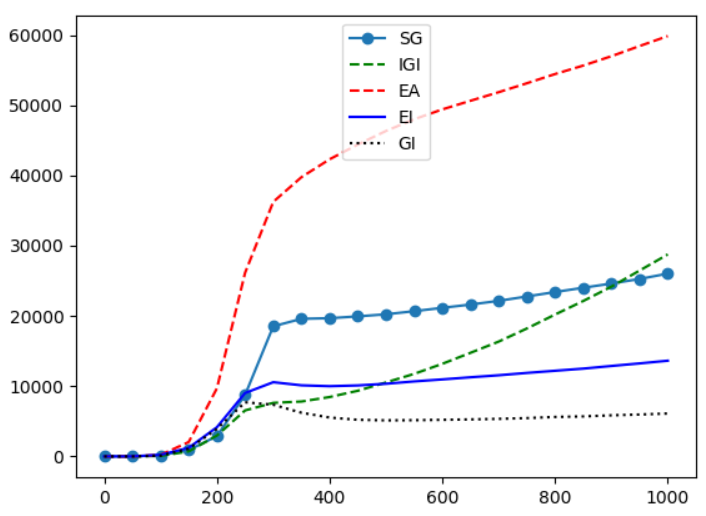
\includegraphics[scale=0.8]{figures/experiments/exp3/mutations}
\caption{Completar.}
\end{figure}

Lorem ipsum dolor sit amet, consectetur adipisicing elit, sed do eiusmod tempor incididunt ut labore et dolore magna aliqua.
Ut enim ad minim veniam, quis nostrud exercitation ullamco laboris nisi ut aliquip ex ea commodo consequat.
Duis aute irure dolor in reprehenderit in voluptate velit esse cillum dolore eu fugiat nulla pariatur.
Excepteur sint occaecat cupidatat non proident, sunt in culpa qui officia deserunt mollit anim id est laborum.

\begin{figure}[h]
\centering
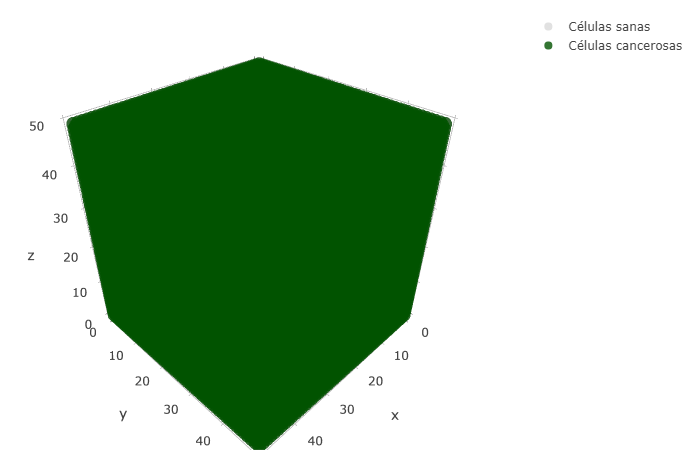
\includegraphics[scale=0.6]{figures/experiments/exp3/grid}
\caption{Completar.}
\end{figure}

Lorem ipsum dolor sit amet, consectetur adipisicing elit, sed do eiusmod tempor incididunt ut labore et dolore magna aliqua.
Ut enim ad minim veniam, quis nostrud exercitation ullamco laboris nisi ut aliquip ex ea commodo consequat.
Duis aute irure dolor in reprehenderit in voluptate velit esse cillum dolore eu fugiat nulla pariatur.
Excepteur sint occaecat cupidatat non proident, sunt in culpa qui officia deserunt mollit anim id est laborum.
